\chapter{Autres exemples LaTeX}
\label{app:more-patterns}

% Cette seconde annexe facultative rassemble d'autres formes : sous-figures,
% notation logique, unités, abréviations et page en paysage. Chaque forme
% s'appuie sur un paquet déjà chargé dans preamble.tex. Conservez ce que le
% mémoire utilise et supprimez le reste, avec son paquet.

\section{Sous-figures et flottants côte à côte}

Utilisez \texttt{subcaption} lorsque plusieurs panneaux partagent un même numéro
de figure. Chaque panneau garde sa légende, et la \cref{fig:subfigures} peut être
citée globalement ou panneau par panneau : la \cref{fig:subfigure-graph} montre
l'entrée et la \cref{fig:subfigure-workflow} le calcul.

\begin{figure}[htbp]
  \centering
  \begin{subfigure}[b]{0.46\linewidth}
    \centering
    \begin{tikzpicture}[
  vertex/.style={circle,draw=LMFINavy,thick,minimum size=8mm,inner sep=0pt},
  edge/.style={-{Stealth[length=2.4mm]},thick,LMFITeal},
  node distance=2.2cm
]
  \node[vertex] (a) {$a$};
  \node[vertex, right=of a] (b) {$b$};
  \node[vertex, right=of b] (c) {$c$};
  \node[vertex, below=1.0cm of c] (d) {$d$};

  \draw[edge] (a) -- (b);
  \draw[edge] (b) -- (c);
  \draw[edge] (c) -- (d);
  \draw[edge] (a) to[bend right=18] (d);
\end{tikzpicture}

    \caption{Graphe d'entrée.}
    \label{fig:subfigure-graph}
  \end{subfigure}\hfill
  \begin{subfigure}[b]{0.46\linewidth}
    \centering
    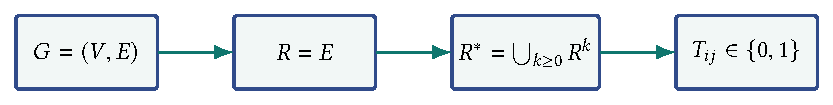
\includegraphics[width=\linewidth]{figures/example-workflow.pdf}
    \caption{Calcul.}
    \label{fig:subfigure-workflow}
  \end{subfigure}
  \caption{Deux vues de l'exemple filé.}
  \label{fig:subfigures}
\end{figure}

Une figure et un tableau peuvent aussi partager une même ligne. Placez chacun
dans une \texttt{minipage} et nommez-les avec \verb|\captionof|, comme pour la
\cref{fig:side-graph} et le \cref{tab:side-edges}.

\begin{figure}[htbp]
  \centering
  \begin{minipage}[c]{0.46\linewidth}
    \centering
    \begin{tikzpicture}[
  vertex/.style={circle,draw=LMFINavy,thick,minimum size=8mm,inner sep=0pt},
  edge/.style={-{Stealth[length=2.4mm]},thick,LMFITeal},
  node distance=2.2cm
]
  \node[vertex] (a) {$a$};
  \node[vertex, right=of a] (b) {$b$};
  \node[vertex, right=of b] (c) {$c$};
  \node[vertex, below=1.0cm of c] (d) {$d$};

  \draw[edge] (a) -- (b);
  \draw[edge] (b) -- (c);
  \draw[edge] (c) -- (d);
  \draw[edge] (a) to[bend right=18] (d);
\end{tikzpicture}

    \captionof{figure}{Le graphe d'exemple.}
    \label{fig:side-graph}
  \end{minipage}\hfill
  \begin{minipage}[c]{0.40\linewidth}
    \centering
    \begin{tabular}{cc}
      \toprule
      De & Vers \\
      \midrule
      $a$ & $b$ \\
      $b$ & $c$ \\
      $c$ & $d$ \\
      $a$ & $d$ \\
      \bottomrule
    \end{tabular}
    \captionof{table}{Sa liste d'arêtes.}
    \label{tab:side-edges}
  \end{minipage}
\end{figure}

\section{Notation logique et informatique}

Les macros du projet se trouvent dans \texttt{macros.tex} : \verb|\N|,
\verb|\Reach| et un délimiteur de crochets sémantiques \verb|\sem|. Avec elles,
\[
  \Reach(u) = \{\, v\in V \mid u\mathrel{R^*}v \,\}, \qquad
  \sem{\varphi}_G \subseteq V, \qquad
  \bigl|\Reach(u)\bigr| \leq n \in \N .
\]
Le paquet \texttt{mathpartir} compose les règles d'inférence ; voici les règles
d'introduction et d'élimination de l'implication, en style séquent :
\begin{mathpar}
  \inferrule*[right=$\to$I]{\Gamma, A \vdash B}{\Gamma \vdash A \to B}
  \and
  \inferrule*[right=$\to$E]{\Gamma \vdash A \to B \\ \Gamma \vdash A}{\Gamma \vdash B}
\end{mathpar}
Les diagrammes commutatifs utilisent \texttt{tikz-cd}. Le carré ci-dessous
commute car toute arête appartient à la clôture : les deux chemins de $E$ vers
$V\times V$ sont l'inclusion de $E$.
\[
  \begin{tikzcd}[column sep=large]
    E \arrow[r, hook] \arrow[d, hook] & R^* \arrow[d, hook] \\
    V\times V \arrow[r, equal] & V\times V
  \end{tikzcd}
\]

% Documentez dans macros.tex chaque macro de notation, et ne définissez que
% celles qui reviennent souvent. Pour les fonctions nommées, déclarez un
% opérateur (\DeclareMathOperator) plutôt que d'employer de simples lettres
% italiques.

\section{Unités, citations et notes de bas de page}

\texttt{siunitx} met en forme nombres et unités selon la langue du mémoire. La
triple boucle de l'\cref{alg:warshall} effectue \num{1073741824} mises à jour
booléennes pour $n=\num{1024}$ ; à \qty{1.5}{\giga\hertz} et une mise à jour par
cycle, cela prend environ \qty{0.72}{\second}. Les citations utilisent
\texttt{csquotes} : \enquote{une citation peut contenir \enquote{une citation
imbriquée}}, avec les guillemets de la langue active. Une note de bas de
page\footnote{Les notes de bas de page sont numérotées en continu dans un chapitre
et composées en bas de page.} reste en dehors de l'argument principal.

\section{Abréviations}

Le paquet \texttt{acro} développe une abréviation à sa première occurrence puis la
raccourcit. Un \ac{dag} n'a aucun cycle orienté, alors que chaque sommet d'une
\ac{scc} atteint tous les autres ; un \ac{dag} en est donc l'extrême opposé. Les
mentions suivantes n'emploient que \ac{dag} et \ac{scc}. Déclarez les abréviations
dans \texttt{macros.tex} ; la liste ci-dessous est produite par
\verb|\printacronyms|.

\printacronyms[heading=none]

\section{Renvois}

Écrivez \verb|\cref| au milieu d'une phrase ; \verb|\Cref| ne sert que pour commencer
une phrase par le nom de l'objet. \texttt{cleveref} ne connaît pas le genre : écrivez l'article devant le renvoi,
comme dans « la \cref{fig:subfigures} », « le \cref{tab:side-edges} », « l'\cref{alg:warshall} »
ou « de l'\cref{eq:transitive-closure} ». Plusieurs objets d'un même type peuvent
être joints : \cref{fig:subfigures,fig:side-graph}. Donnez à chaque étiquette un
préfixe court (\texttt{fig:}, \texttt{tab:}, \texttt{eq:}, \texttt{thm:}) et ne citez
que les objets dont le texte parle.

\clearpage
\begin{landscape}
\section{Un tableau large sur une page en paysage}

Un tableau trop large pour la zone de texte peut être placé sur une page tournée
avec \texttt{pdflscape} ; les visionneuses affichent la page pivotée, tout comme
la copie imprimée. Le \cref{tab:landscape} donne la taille de la matrice booléenne
et le nombre de mises à jour de la triple boucle pour des graphes de plus en plus
grands.

\begin{table}[htbp]
  \centering
  \caption{Entrées de la matrice et mises à jour booléennes de l'\cref{alg:warshall} pour $n$ sommets.}
  \label{tab:landscape}
  \small
  \begin{tabular}{@{}l *{9}{r}@{}}
    \toprule
    $n$ & \num{4} & \num{8} & \num{16} & \num{32} & \num{64} & \num{128} & \num{256} & \num{512} & \num{1024} \\
    \midrule
    Entrées $n^2$ & \num{16} & \num{64} & \num{256} & \num{1024} & \num{4096} & \num{16384} & \num{65536} & \num{262144} & \num{1048576} \\
    Mises à jour $n^3$ & \num{64} & \num{512} & \num{4096} & \num{32768} & \num{262144} & \num{2097152} & \num{16777216} & \num{134217728} & \num{1073741824} \\
    \bottomrule
  \end{tabular}
\end{table}

% N'utilisez une page en paysage que si un tableau ou une figure ne peut pas
% être rendu lisible en portrait : réduisez d'abord la police ou scindez le
% tableau. Tout objet en paysage a la même légende et le même renvoi que
% n'importe quel flottant.
\end{landscape}
